\section{Referencial Teórico}\label{sec:referencial-teorico}

Nesta Seção, os principais conceitos relacionados a este trabalho são apresentados, fornecendo subsídios para o desenvolvimento do projeto de detecção de pessoas em ambiente fechado, usando mapas de profundidade. A subseção \ref{sec:deteccao-rastreamento} apresenta conceitos relacionados à detecção e rastreamento de pessoas. A subseção \ref{sec:tec-rastreamento} discute o tópico tecnologias de rastreamento. Por fim, na subseção \ref{sec:determ-posic} são abordadas as técnicas de determinação de posição comumente utilizadas. \textcolor{red}{REVER esse paragrafo, atualizando-o ao final da edição dessa seção. EX: tecnologias de rastreamento devem ser exluidas.}


\subsection{Biometria e Sistemas Biométricos}\label{sec:biometria}
O termo biometria deriva do grego bios (vida) + metron (medida) e, na autenticação, refere-se à utilização de características próprias de um indivíduo para proceder à sua autenticação e/ou identificação \cite{magalhaes2003biometria}. Na biometria utiliza-se caracteristicas fisicas/fisiológicas ou comportamentais para a identificação de pessoas, sendo baseada em algo que a pessoa e e não em algo que ela possui ou sabe. A Figura~\ref{fig:biometria} ilustra exemplos de características biométricas \cite{cardia2015avaliaccao}.

\begin{figure*}[ht]
\centering
    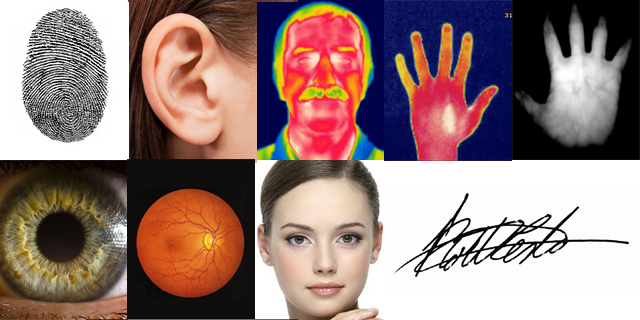
\includegraphics[resolution=300,width=0.7\textwidth,natwidth=610,natheight=642]{images/biometria.png}
    \caption{Exemplos de características biométricas: impressão digital, orelha, termograma facial, termograma da mão, padrões de veias da mão, íris, retina, face e assinatura.}
    \label{fig:biometria}
\end{figure*}

Características fisicas/fisiológicas são baseadas na anatomia ou no funcionamento do organismo de uma pessoa viva, como impressão digitalou termograma facial. Já as comportamentais são baseadas na forma particular que um sujeito executa uma ação, como o a dinâmica de digitação ou a assinatura captada de modo digital. Qualquer característica pode ser utilizada desde que atenda algumas restrições, tais como \cite{maltoni2009handbook}:

\begin{itemize}
\item Universalidade: A característica deve estar presente na maior quantidade possível de pessoas;
\item Unicidade: A característica deve ser diferente entre pessoas diferentes;
\item Permanência: A característica não deve mudar com o passar do tempo;
\item Mensurabilidade: A característica deve ser fácil de coletar e mensurar;
\item Desempenho: A característica deve permitir alta acurácia com baixo tempo de processamento e custo computacional, além de ser robusta a ambientes não controlados;
\item Aceitabilidade: A característica deve ser aceita facilmente pelas pessoas como forma de identificação;
\item Grau de impostura: A característica deve ser resistente a fraude.
\end{itemize}

Um sistema de reconhecimento de padrões que utiliza um vetor de característica baseado em qualquer traço biométrico para garantir a identidade de uma pessoa é um sistema biométrico. Esses sistemas recebem a característica da pessoa, e processa em uma forma reduzida chamada de \textit{template}. Esse \textit{template} pode ser armazenado em um banco de dados central ou em um dispositivo de mídia removível.Segundo Wayman \cite{wayman2002}, um sistema biométrico pode ser classificado em uma das setes categorias: 

\begin{itemize}
\item Cooperativo ou não cooperativo: O sujeito deseja ser identificado?
\item Evidente ou sigiloso: O sujeito sabe que ele está sendo identificado?
\item Habituado ou não habituado: O sujeito frequentemente se submete a identificação?
\item Auxiliado ou não auxiliado: Existe um operador humano auxiliando o sistema?
\item Ambiente controlado ou não controlado: Em qual ambiente o sistema irá operar?
\item Privado ou público: Os sujeitos são empregados (privado) ou clientes (público)?
\item Aberto ou fechado: O sistema precisa de padrões para ter interoperabilidade entre sistemas?
\end{itemize}




\subsection{Detecção, identificação e rastreamento}\label{sec:deteccao-rastreamento}

As aplicações de localização interior têm experimentado esforços adicionais nos últimos anos com o aparecimento da computação ubíqua. Em vários cenários, objetos e mercadorias devem estar localizados ou monitorados, por exemplo, em um ambiente industrial ou médico. Adicionalmente, a localização de pessoas permite a criação de uma série de aplicativos e serviços. Clientes e funcionários podem ser observados, invasores detectados, idosos assistidos, e pacientes acompanhados. Em locais públicos, como estações de metrô, as preocupações de segurança podem ser abordadas por um sistema de orientação de emergência \cite{linde2006aspects}. 

Segundo Jaeseok Yun e Sang-Shin Lee \cite{yun2014human}, um sistema de controle de movimentos deve detectar robustamente: 
\begin{itemize}
  \item A identidade do objeto em movimento;
  \item Em qual o local está o objeto; 
  \item Em que sentido o objeto está se movimentando;
  \item O quão rápido esse objeto se move. 
 \end{itemize}

Uma das questões-chave da emergente computação móvel e robótica é a obtenção do conhecimento da posição de pessoas e objetos em um ambiente interno \cite{linde2006aspects}. A fim de construir um ambiente inteligente, onde os sistemas possam entender as atividades nas quais o usuário está envolvido e suas imediações, para então adaptar os seus serviços e recursos para o contexto do usuário, é necessário desenvolver um sistema de detecção, identificação e rastreamento de movimento robusto usando vários sensores \cite{yun2014human}. Esses três conceitos serão discutidos a seguir.


\subsubsection{Detecção de pessoas}\label{sec:deteccao-movimento}
 
 \textcolor{red}{essa subsecao está pobre}
 
\subsubsection{Identificação de indivíduos}\label{sec:identificacao-pessoas}

Sistemas de sensores para identificação recolhem um conjunto de dados brutos do corpo humano, bem como extraem características distintas visando reconhecer o contexto principal: a identidade do objeto \cite{yun2014human}. Para esse fim, inúmeros sistemas têm sido estudados usando vários sensores, incluindo câmeras, sensores de movimento, blocos de pressão, radares, sensores de campo elétrico, etc.
\textcolor{red}{essa subsecao está pobre}
 
\subsubsection{Rastreamento de pessoas}\label{sec:rastre-amb-fec}

 \textcolor{red}{essa subsecao está pobre}

\subsection{Tecnologias de detecção Visuais, não visuais e combinadas}\label{sec:tec-rastreamento}
No geral, sistemas de monitoramento podem ser não visuais, visuais (com ou sem a utilização de marcadores) ou uma combinação de ambos \cite{zhou2008human}.

\subsubsection{Tecnologias visuais}\label{sec:sens-genericos}
Muitos pesquisadores têm dedicado os seus esforços para a construção de sistemas de detecção de movimento robustos usando sensores baseados na visão usando câmeras. Os projetos de investigação com base em sensores baseados em visão consideram, principalmente, posição, velocidade, direção, forma e tamanho (ou seja, o número de \textit{pixels} em câmeras) como o contexto principal para identificar os usuários e compreender as suas atividades \cite{stauffer200l}.

Existem duas principais técnicas no acompanhamento visual do movimento humano: rastreamento baseado marcador e rastreamento livre de marcador \cite{YTao2010}.

Rastreamento visual com marcador base (\textit{Visual marker based tracking}) é uma técnica onde as câmeras são utilizadas para controlar os movimentos humanos. São adicionados identificadores sobre o corpo humano. Devido ao fato de o esqueleto humano ser uma estrutura altamente articulada, torções e rotações podem gerar movimento muito complexos. Como consequência, cada parte do corpo realiza uma trajetória de movimento imprevisível e complicada, o que pode levar a estimativa de movimento inconsistente e pouco confiável. Além disso, cenas desordenadas, ou variação de iluminação podem distrair a atenção visual a partir da posição real de um marcador. Como uma solução para esses problemas, o rastreamento visual com marcador base é preferível nestas circunstâncias \cite{zhang2002visual}.

Entretanto, essas tecnologias possuem limitações as quais podem apresentar falhas devido:

\begin{enumerate}
    \item A identificação dos pontos ósseos padrões pode não ser confiável; 
    \item O tecido macio que se sobrepõe pontos ósseos podem mover-se, dando origem a dados ruidosos; 
    \item O próprio marcador pode oscilar devido à sua própria inércia; 
    \item Marcadores podem mesmo vir à deriva completamente.
\end{enumerate}

Sistemas visuais de rastreamento livres de marcador (\textit{Marker-free visual based tracking systems}) somente exploram sensores óticos para medir o movimentos do corpo humano. Esta aplicação é motivada pelas falhas do uso de sistemas baseados em marcador visual, anteriormente apresentadas. 
 \textcolor{red}{essa subsubsubsubsubsecao está pobre}



\subsubsection{Tecnologias não visuais}\label{sec:tec-vis}
Sensores utilizados nestes sistemas interagem direta ou indiretamente com o corpo humano a fim de recolher informações relativas ao movimento. Estes sensores são comumente classificados como mecânicos, inerciais, envoltório acústico, rádio ou micro-ondas e com base magnética \cite{zhou2008human}. De um modo geral, cada tipo de sensor tem as suas próprias vantagens e limitações. Limitações de modalidade específica, medição específica, e circunstâncias específicas afetam, consequentemente, o uso de tipos particulares de sensores, em ambientes diferentes \cite{Welch:2002}.

\subsubsection{Tecnologias combinadas de rastreamento}\label{sec:rastre-robo}
Estes sistemas tiram proveito das vantagens das tecnologias visuais e não visuais. Essa estratégia de combinação ajuda a reduzir erros decorrentes da utilização de plataformas individuais. Por exemplo, os limites ou silhuetas de partes do corpo humano podem ser capturados em uma trajetória de movimento, se marcadores montados sobre essas partes não estão no "campo de visão" das câmeras. Essa estratégia exige calibração e computação intensivas \cite{zhou2008human}.

\subsection{Técnicas de determinação de posição}\label{sec:determ-posic}
Por natureza, o posicionamento é um problema interdisciplinar que traz consigo inúmeras questões em vários campos de pesquisa, como engenharia, ciência da computação e estatística. Como consequência, a concepção e implementação de um sistema de localização é uma tarefa bastante complexa que implica um entendimento nesses domínios \cite{linde2006aspects}. 

\subsubsection{Posição física e localização simbólica}\label{sec:posic-fisica}
A localização simbólica, ou posicionamento relativo, descreve o procedimento de determinação da posição atual de um alvo móvel usando o curso e a velocidade da informação. Pode ser subdividida em duas abordagens: odometria e navegação inercial \cite{linde2006aspects}.

Odometria é uma abordagem avançada para estimar navegação. Começando a partir de uma posição conhecida, a presente localização de uma unidade pode então ser determinada por meio da reconstrução do caminho percorrido. A odometria é totalmente autossuficiente mas, por outro lado, está sujeita a erros. Esses erros podem ser sistemáticos, como por exemplo erros causados por diâmetros desiguais ou desalinhamento das rodas, ou não sistemáticos, como por exemplo movimento sobre solos não uniformes ou sobre obstáculos inesperados. 

Sistemas de navegação inercial (INS) usam giroscópios e acelerômetros para medir a velocidade de rotação e aceleração de uma unidade. A Informação sobre a posição é calculada mediante a integração dos dados medidos duas vezes. Assim como os sistemas de odometria, os sistemas de navegação inercial são autossuficientes, mas estão susceptíveis aos mesmos erros que podem ocorrer em sistemas de odometria. Um sistema inercial pode ajudar a compensar erros de odometria momentâneas \cite{linde2006aspects}.

A posição física, ou absoluta, de uma unidade móvel pode ser determinada com a ajuda de pontos de referência fixos localizados no ambiente. A posição destes pontos de referência é conhecida a priori e essas referências podem ser componentes ativos ou passivos. Esta técnica apresenta três abordagens: registro de balizas, ponto de referência e modelo de harmonização \cite{linde2006aspects}.

Balizas ativas são componentes estáticos localizados em posições fixas e conhecidas do ambiente. Existem dois tipos diferentes de balizas: balizas auto atuantes que emitem periodicamente certa assinatura (por exemplo, uma sequência de \textit{bits} única), e balizas sensíveis. Balizas sensíveis podem atuar como ouvintes ou ativamente refletir uma assinatura recebida emitida pela unidade móvel. Ponto de referência são características estáticas de um ambiente que podem ser reconhecidos por uma unidade móvel. Na maioria das vezes, esses marcos são formas geométricas, como retângulos, linhas ou códigos de barras. Além desses objetos artificiais, itens naturais, como portas também podem servir como pontos de referência. Além disso, a análise geral da cena é frequentemente utilizada neste contexto. No modelo de harmonização, uma unidade móvel deve ser capaz de construir um mapa ou modelo de um ambiente desconhecido e, ao mesmo tempo localizar-se no interior deste mapa. Enquanto se move e explora, um modelo de referência é criado. O posicionamento é realizado comparando este modelo de referência (possivelmente pré-armazenado) a um modelo local gerado a partir dos dados dos sensores a bordo \cite{linde2006aspects}.

\subsubsection{Trilateração}\label{sec:trilat}
A trilateração é uma técnica para calcular uma posição de um objeto $m$, tendo suas distâncias $l_{am}$, $l_{bm}$ e $l_{cm}$ para três objetos de referência não colineares\footnote{ Cálculo para um cenário 2D. A localização em 3D requer quatro referências não coplanares} fixos $a, b$ e $c$ (ver Fig.~\ref{fig:trilateracao}). Para cada distância $l_{pm}$ entre $m$ e $p$ (com $p \in \{a, b, c\}$), um círculo em ($x_{p}, y_{p}$) com raio $l_{pm}$ pode ser desenhado em torno de $p$. O ponto de interseção de três desses círculos produz as coordenadas ($x_{m}, y_{m}$) de $m$. Portanto, a trilateração pode ser expressa como encontrar a solução para o seguinte sistema de equações quadráticas \cite{linde2006aspects}:

\begin{align*}
(x_{m}-x_{a})^{2} + (y_{m}-y_{a})^{2} = {l_{am}}^{2}\\
(x_{m}-x_{b})^{2} + (y_{m}-y_{b})^{2} = {l_{bm}}^{2}\\
(x_{m}-x_{c})^{2} + (y_{m}-y_{c})^{2} = {l_{cm}}^{2}
\end{align*}



 \begin{figure}[ht]
\centering
    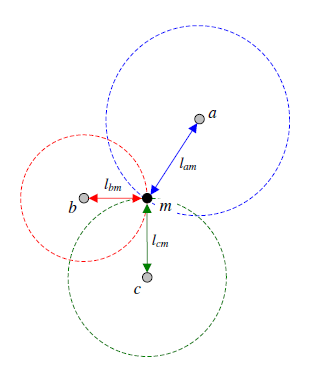
\includegraphics[resolution=300,width=0.4\textwidth,natwidth=610,natheight=642]{images/trilateracao.png}
    \caption{Esquema de Trilateração.}
    \label{fig:trilateracao}
\end{figure}

\subsubsection{Triangulação}\label{sec:triang}


A localização baseada na trilateração implica que os participantes devem ser capazes de medir distâncias (ou diferenças de distância) entre si. A triangulação funciona de forma semelhante, mas em vez de distâncias, os ângulos são medidos. De fato, pode-se demonstrar que a triangulação pode ser transformada em trilateração por meios simples\cite{linde2006aspects}. 

Triangulação requer a medição de ângulos entre as unidades de referência fixas e o alvo móvel. As unidades móveis calculam os ângulos em direção aos sinais emitidos por unidades fixas de referência. Obtém-se então a posição e orientação através dos dados recolhidos. As unidades de referência medem os ângulos na direção do sinal emitido pela unidade móvel. Apenas uma estimativa da localização, mas não a orientação do alvo móvel, pode ser obtida \cite{lutzke2013experimental}. Dois casos podem ser distinguidos, conforme ilustrado na Fig.~\ref{fig:triang}:


\begin{itemize}
  \item A unidade móvel mede os ângulos em direção a sinais emitidos por unidades de referência fixas (ver Fig.~\ref{fig:triang}(a)). Os dados recolhidos fornecem a posição e orientação.
  \item As unidades de referência medem ângulos em direção ao sinal emitido pela unidade móvel (ver Fig.~\ref{fig:triang}(b)). Apenas uma estimativa de localização, mas não a orientação do alvo móvel, pode ser obtida.
 \end{itemize}


\begin{figure*}[ht]
\centering
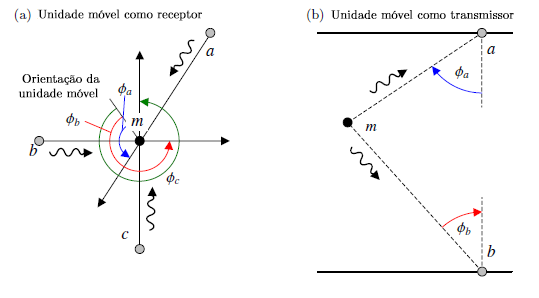
\includegraphics[resolution=300,width=0.7\textwidth,natwidth=610,natheight=642]{images/triangulacao.png}
    \caption{Esquemas de triangulação.}
    \label{fig:triang}
\end{figure*}
 
\subsubsection{Proximidade e análise de cena}\label{sec:proximidade}
Outra abordagem de localização é a técnica de detecção de proximidade na qual a posição de um alvo é aproximada, selecionando a localização da unidade de referência mais próxima. Por conseguinte, não é necessário cálculo de localização. Alternativamente, se várias unidades de referência estão dentro do alcance, o baricentro entre estas unidades podem produzir uma melhor estimativa \cite{EHuber1996}.
 \textcolor{red}{essa subsubsubsubsubsecao está pobre. DETALHAR detecção de proximidade, incluindo calculos.}

Pontos de referência (\textit{Landmarks}) são elementos estáticos de um ambiente que pode ser reconhecido por uma unidade móvel. Na maioria das vezes, os pontos de referência são formas geométricas, como retângulos, linhas ou códigos de barras. Itens naturais, como portas podem também servir como pontos de referência. O termo  análise de cena é frequentemente utilizado neste contexto. Unidades móveis tentam localizar-se  em determinado ambiente usando a visão da câmera, bem como funcionalidades de extração para analisar o cenário atual. Uma vez que um marco foi reconhecido e identificado de forma confiável, a posição atual da unidade em relação ao marco correspondente pode ser calculada. Isto é conseguido através de triangulação, trilateração e proximidade \cite{linde2006aspects}.
 
 \subsection{Kinect}\label{sec:kinect}
 
O Kinect (Fig.~\ref{fig:kinect}) é um sensor de movimento, projetado pela Microsoft Inc. e lançado em novembro de 2010 para ser usado como controle remoto para o console de videogames Xbox 360. É composto por vários sensores (Fig. ~\ref{fig:kinect}): Uma câmera RGB (Color CMOS, VNA38209015), uma câmera de profundidade composta por um projetor de infravermelho (OG12 / 0956 / D306 / JG05A) combinado a uma câmera de infravermelho (IR CMOS, Microsoft / X853750001 / VCA379C7130) e uma série de quatro microfones. A câmera infravermelha e a câmera colorida têm uma definição de 640 x 480 pixels. O ângulo de visão é $60\,^{\circ}$ horizontal e $45\,^{\circ}$ vertical. O dispositivo foi projetado para ser usado em uma faixa de 0,5 m a 5 m \cite{sevrin2015characterization}. A tabela \ref{table:comparativoScanners} apresenta um comparativo entre o Kinect e os \textit{scanners} 3D mais utilidados.

 \begin{figure}[h]
\centering
    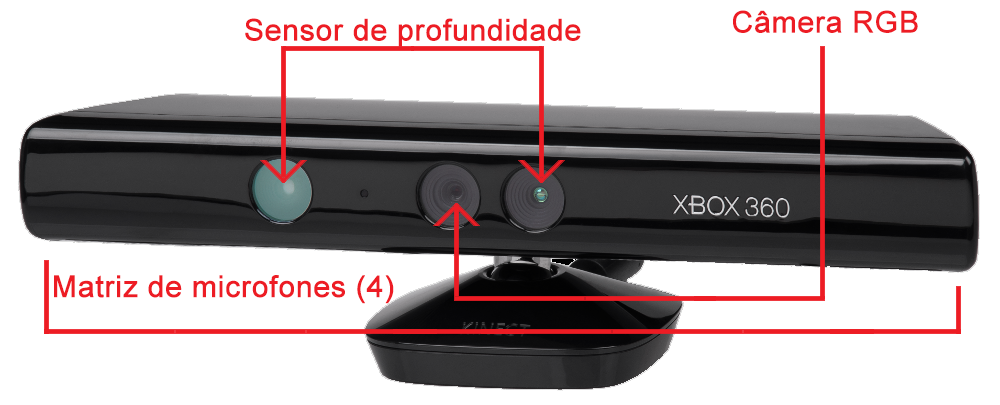
\includegraphics[resolution=300,width=0.4\textwidth,natwidth=610,natheight=642]{images/kinect.png}
    \caption{O Sensor Microsoft Kinect.}
    \label{fig:kinect}
\end{figure}


 \begin{table}[h]
 \caption{Comparação entre diferentes \textit{scanners} 3D \cite{li2013using}.\newline A velocidade é expressada em segundos, tamanho em polegadas, preço em USD e a acurácia é uma aproximação expressada em mm.}
 \label{table:comparativoScanners}
 \begin{tabular}{|l|c|c|c|c|c|}
\hline  
 Dispositivo & Velocidade & Carga & tamanho & Preço & Acurácia \\ \hline  
 3dmD & 0.002 & 10 s & N/A & >\$50k & <0.2 \\ \hline  
 Minolta & 2.5 & Não & 1408 & >\$50k & 0.1 \\ \hline  
 Artec Eva & 0.063 & Não & 160.8 & >\$20k & 0.5 \\ \hline  
 3D3 HDI R1 & 1.3 & Não & N/A & >\$10k & 0.3 \\ \hline  
 SwissRanger & 0.02 & Não & 17.53 & >\$5k & 10 \\ \hline  
 David SLS & 2.4 & Não & N/A & >\$2k & 0.5 \\ \hline  
 Kinect & 0.033 & Não & 41.25 & >\$200k & 1.5-50 \\ \hline
\end{tabular}
\end{table}


\textcolor{red}{como que tudo isso que vc escreveu nessa secao se relacionada ao seu trabalho? o que vc usará? é sempre bom ir deixando claro isso.}


 Neste trabalho, será apresentada uma nova abordagem sensorial: associação de Técnicas Visuais e Não Visuais para a detecção \textcolor{red}{alinhe isso com o seu título. lá vc fala de identificacao e rastreamento, aqui vc diz deteccao. novamente misturando os conceitos. seja conciso nisso} de presença em um ambiente interno \cite{yun2014human}.